% ~ 12 pages
\chapter{Identification of Hadronic Tau Lepton Decays using Neural Networks}
\label{sec:rnn}

This chapter investigates the application of neural networks for tau
identification. First it will be shown that a multi-layer perceptron (MLP) can
achieve a classification performance comparable to the optimised BDT from the
previous chapter. Subsequently, novel sequence learning techniques are employed
to create classifiers operating on sequences of reconstructed objects. For this
the recurrent neural networks based on the LSTM architecture are used to create
classifiers operating on tracks in the inner detector and clusters in the
calorimeter. In this context a tau identification algorithm using purely
calorimetric information is developed and its potential application for reducing
the trigger-rate of a di-tau trigger at the \emph{High Luminosity LHC} (HL-LHC)
is presented. Finally, a model combining the multi-layer perceptron and the
recurrent networks operating on track- and cluster-information is developed.

\section{Identification using Feedforward Neural Networks}
\label{sec:ffnn_id}

Before proceeding to sequence classification techniques the viability of neural
networks to perform tau identification using simple network architectures is
shown. This will aid as a introduction to important concepts when training
neural networks. Moreover, the resulting network will be used as a building
block in the final model.

The optimised BDT from Chapter~\ref{sec:bdt} will be used as a reference for the
investigations in this chapter. Therefore the models will be trained and
evaluated using the same event samples, preselection and reweighting scheme
presented in Section~\ref{sec:bdt_eventsim}. In contrast to hold-out validation
used in the previous chapter, the full event sample is now randomly split into a
training, validation and testing sample. The samples have a relative size of
\SI{40}{\percent}, \SI{10}{\percent} and \SI{50}{\percent}, respectively. The
purpose of the training and testing sample is the same as before, however the
validation sample is monitored during the training process and used to perform
model selection and early stopping. A separate sample, as opposed to the testing
sample, is used to avoid introducing biases in the performance measurement on
the testing sample. This approach will be used for the remainder of this
chapter.

To reproduce the performance of the BDT-based tau identification a multi-layer
perceptron (MLP) with two hidden layers~(cf.\ Section~\ref{sec:nn_feedforward})
is used. The MLP uses the same input variables used for the optimised BDT.
Moreover, the input variables are standardised by subtracting the mean and
dividing by the standard deviation derived from the distributions in the
training sample. This preprocessing step is important as the gradient descent
algorithm used for training is sensitive to variables on different scales. The
input layer of the MLP consists of 9 (10) neurons corresponding to the input
variables for the 1-prong (3-prong) identification. Both hidden layers of the
MLP have a size of 128 units, which are activated by rectified linear units
(ReLU). A single output neuron using the logistic sigmoid as its activation
function, therefore returning probabilities of an event being signal-like. The
binary cross-entropy loss function is used and minimised by the \emph{Adam}
optimiser.

\begin{figure}[htb]
  \begin{subfigure}[t]{0.48\textwidth}
    \centering
    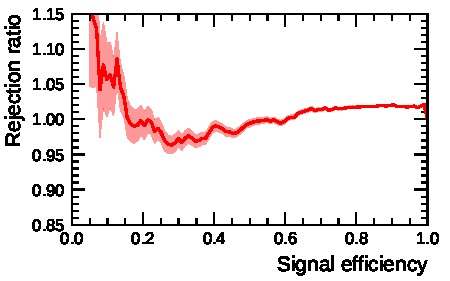
\includegraphics{./figures/rnn/mlp/mlp_bdt_ratio_1p.pdf}
    \subcaption{1-prong}
  \end{subfigure}\hfill
  \begin{subfigure}[t]{0.48\textwidth}
    \centering
    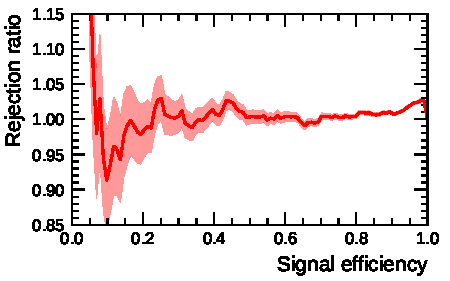
\includegraphics{./figures/rnn/mlp/mlp_bdt_ratio_3p.pdf}
    \subcaption{3-prong}
  \end{subfigure}
  \caption{Ratio of background rejection of the MLP and the optimised BDT as a
    function of signal efficiency. The band indicates the $1\sigma$-interval.}
  \label{fig:roc_mlp_bdt_comparison}
\end{figure}

In Figure~\ref{fig:roc_mlp_bdt_comparison} the ratio of rejection of the MLP and
the optimised BDT is depicted as a function of the signal efficiency. The
1-prong MLP shows comparable performance above \SI{60}{\percent} signal
efficiency, which approximately corresponds to the tight working point. Over the
intermediate efficiency range the performance degrades slightly. The 3-prong MLP
is consistent with the performance of the optimised BDT identification with a
small improvement at high efficiencies.

To summarise, both the 1- and 3-prong MLP achieve similar performance
characteristics as the optimised BDT from Chapter~\ref{sec:bdt}. The results
show that neural networks are a viable method to perform tau identification.

\section{Identification using Recurrent Neural Networks}
\label{sec:rnn_id}

Thus far approaches of tau identification use high-level variables that
summarise properties of reconstructed objects in the detector. This has the
advantage that identification can be understood and investigations into
systematic errors are simplified. However, discriminative power can be lost when
transitioning from low- to high-level variables. Therefore an approach is
presented capturing low-level information by employing sequence classification
techniques. A general description of the method is given and subsequently
applied to reconstructed tracks and clusters in the calorimeter.

\subsection{Motivation and General Description}
\label{sec:rnn_descr}

The variable importance of the BDT-based tau identification in
Section~\ref{sec:bdt_var_importance} showed that a large fraction of the
background rejection can be attributed to variables derived from tracking
information. Examples are the variables sensitive to the decay length of the tau
lepton~$|S_\text{leadtrack}|$ and $S_\text{T}^\text{flight}$ as well as the
transverse momentum fraction of isolation tracks~$f_\text{iso}^\text{track}$ and
the mass of the track system~$m_\text{track}$. Moreover, during the preparation
of the tau identification for the ATLAS reconstruction release to be used for
the remainder of Run-II, it was observed that tracks classified as
\emph{isolation}, i.e.\ primary particle tracks not originating from the tau
decay, offer discriminative power against tau candidates from multijet events.
However, instabilities of the \emph{isolation} track category lead to the
necessity to decouple tau identification and the track classification by
introducing the \emph{modified isolation} category. This lead to an average
rejection loss of the order of \SI{20}{\percent} for the 1-prong identification,
while the 3-prong identification was not significantly affected. Therefore, the
aim is to improve the use of isolation information in reconstructed tracks of a
hadronic tau decay.

\begin{figure}[htb]
  \centering
  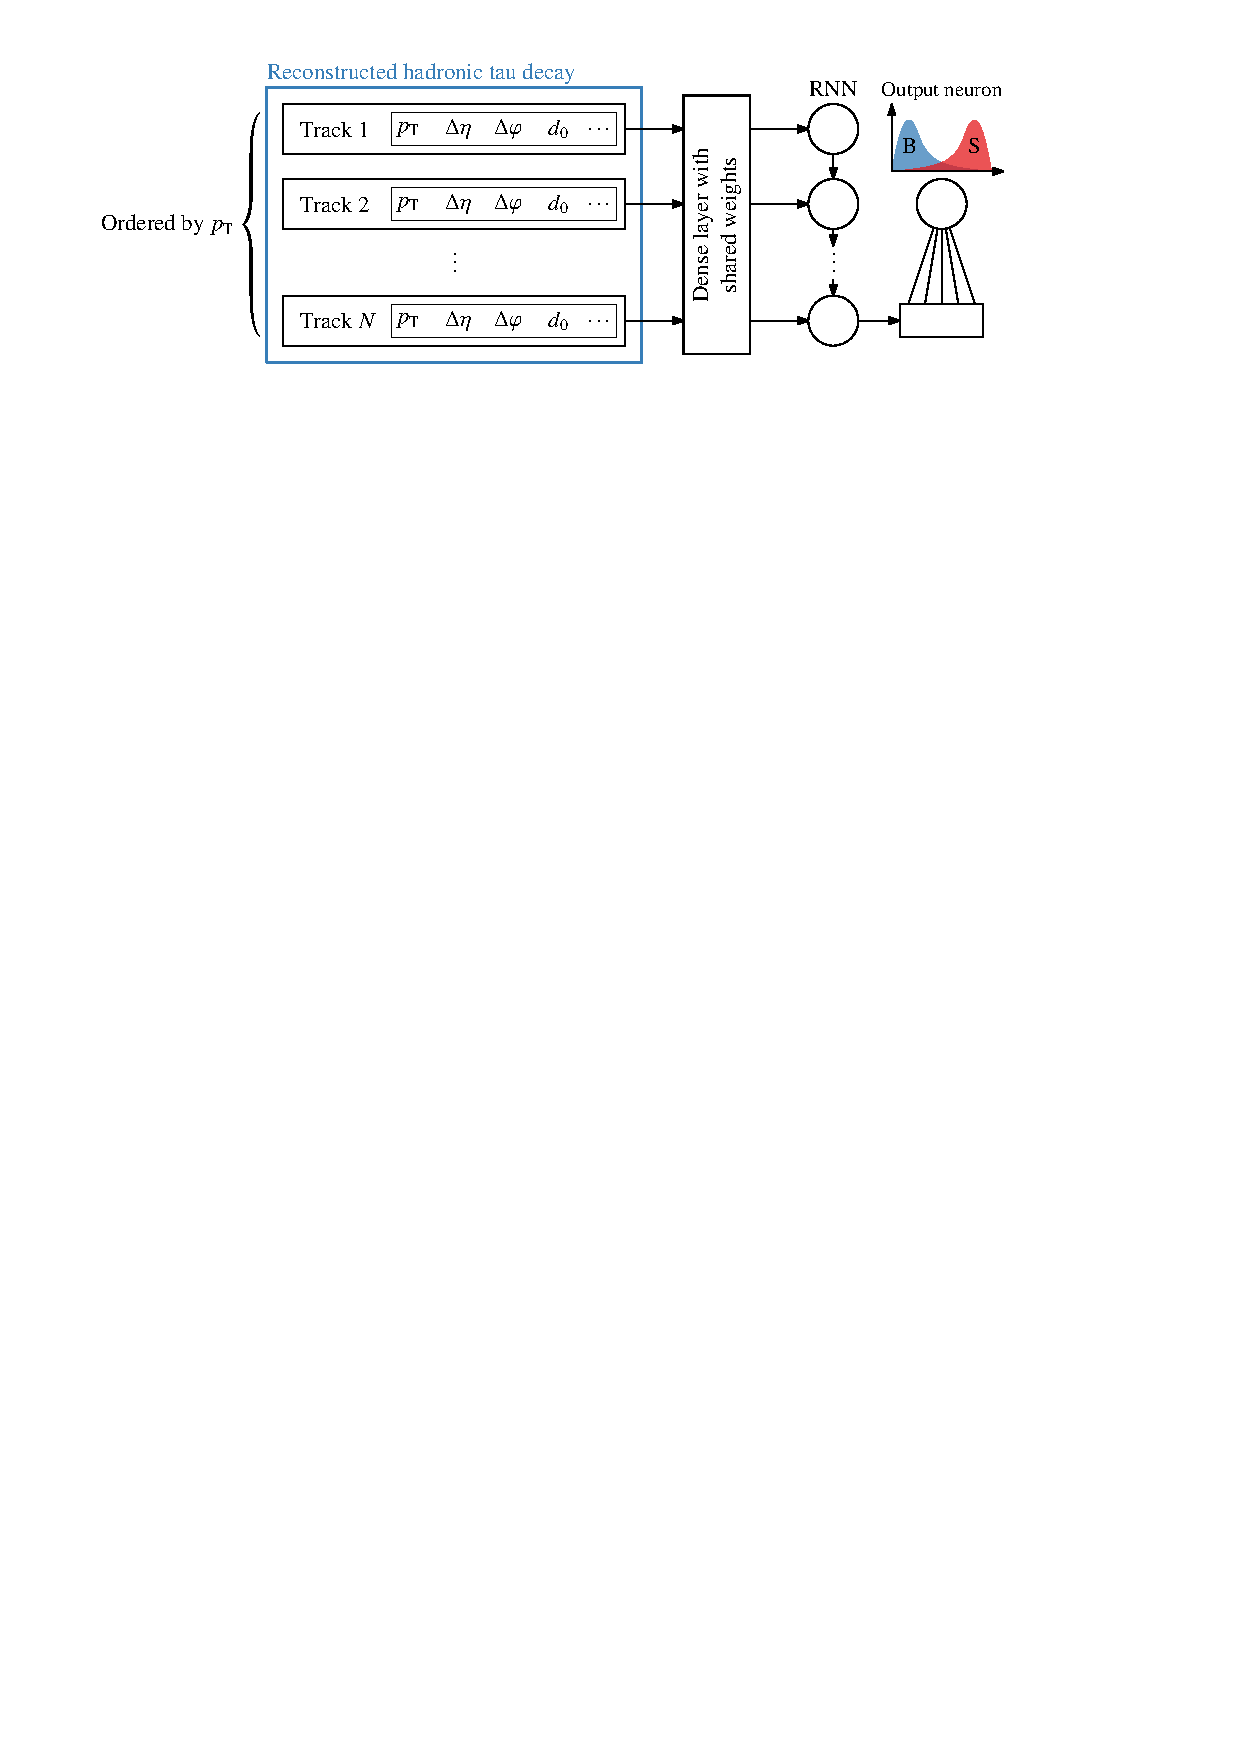
\includegraphics[scale=0.9]{./figures/rnn/track_rnn_schematic.pdf}
  \caption{Schematic description of a recurrent neural network using individual
    tracks for tau identification.}
  \label{fig:track_rnn_schematic}
\end{figure}

For this purpose recurrent neural networks using the LSTM architecture are used
to classify a sequence of objects reconstructed in the detector. The following
will focus on describing the method using tracks in the ID but the use of other
physics objects is analogous. Figure~\ref{fig:track_rnn_schematic} describes the
architecture used in this chapter. Reconstructed hadronic tau decays have a
number of associated tracks, which can be interpreted as elements in a sequence.
Each track in the sequence has variables related to the properties of the track,
e.g.\ the transverse momentum of the track. Moreover, the elements can also be
assigned global information about the tau decay, e.g.\ the visible transverse
momentum of the tau. The sequence of tracks is sorted according to a
well-defined and physically motivated ordering scheme. For the RNN using track
information a descending~$p_\text{T}^\text{track}$ ordering is used. In practice
the maximum sequence length is limited by truncation.

The tracks and the values of their input variables are passed in the predefined
order to a dense layer with shared weights. This layer applies a transformation
on the variables of each individual track, where the parameters of this
transformation are shared between each element in the sequence. It creates a
sequence of intermediate representations of the tracks, which are then passed to
the recurrent layer employing the LSTM architecture. The output of the final
time step of the RNN, consisting of a vector of activations, is passed to a
dense layer with one neuron and logistic sigmoid activation. The activation of
the output neuron can then be used to classify the tau candidate as signal or
background.

\subsection{Track-RNN}
\label{sec:rnn_tracks}
\todo[inline]{Better name for this section.}

The implementation of the RNN employing track information, hereafter abbreviated
as Track-RNN, uses tracks associated with a reconstructed tau, which are tracks
in the $\Delta R < 0.4$ cone passing a transverse momentum threshold of
\SI{400}{\MeV} from track reconstruction. The variables attached to each track
are summarised in the following:
\begin{description}
\item[Transverse momentum of track and jet] The transverse momentum of the
  track~$p_\text{T}^\text{track}$ as measured in the tracking system is used.
  The inclusion of the track momentum is crucial as it allows the network to
  discriminate between tracks originating from the hard scattering and soft
  processes. Additionally, the transverse momentum of the anti-$k_\text{t}$ jet
  used to seed the tau candidate~$p_\text{T}^\text{jet}$ is appended to the
  input variables of each track.
  \todo[inline]{Why jet seed instead of tau at LC scale?}

\item[Impact parameters w.r.t.\ the tau vertex] The transverse~$d_0$ and
  longitudinal impact parameters~$z_0 \sin\theta$ (distance of closest approach
  in the $z$-$r$ plane) with respect to the associated primary vertex of the tau
  decay is used. The longitudinal impact parameter is multiplied
  by~$\sin\theta$, where~$\theta$ is the azimuthal angle of the track
  parametrisation, to account for larger errors of~$z_0$ for tracks in the
  forward region. Impact parameter information is important to determine whether
  a given track originated from the tau vertex. It allows to discriminate
  between tracks from the tau decay or jet and tracks from other interactions
  during the same bunch crossing.

\item[Angular distance to the tau axis] The signed angular distance of the track
  to the tau axis in the longitudinal~$\Delta \eta$ and transverse
  plane~$\Delta \varphi$. The angular distances allow probing the spacial
  isolation of the tracks in a tau decay.

\item[Track quality criteria] The Track-RNN includes basic track quality
  criteria to allow to reject tracks of low reconstruction quality. Therefore,
  the number of hits in the pixel layers~$N_\text{Pixel}$ and semiconductor
  tracker~$N_\text{SCT}$ are used.
  % IBL TOO!

\item[Electron probability] The probability of the track originating from an
  electron estimated using high-threshold hit information in the
  TRT~$p_\text{HT}$. It is used to identify tracks originating from photon
  conversion.
\end{description}
Including the track category from the multivariate track classification was also
investigated leading to a small improvement in discrimination power. It is not
included in favour of decoupling the tau identification from track
classification.

Basic transformations are applied to the input variables to make them mroe
appropriate for the use in neural networks. Therefore, the transverse
momenta~$p_\text{T}^\text{track}$ and $p_\text{T}^\text{jet}$ are
log-transformed. Moreover, only the absolute value of the impact parameters is
used, which is also log-transformed. Similar to the MLP the input variables have
to be standardised. For transverse momenta and impact parameters this is done by
subtracting an offset and dividing by a scale factor. The offset is the mean of
the corresponding quantity in tracks of the training sample and the scale factor
the corresponding standard deviation. Angular distances are scaled into the
$[-1, 1]$-interval and similarly the number of hits in the inner detector
into~$[0, 1]$. The training process is analogous the the MLP and not repeated
here.

The size of the layers in the architecture depicted in
Figure~\ref{fig:track_rnn_schematic} is optimised by observing the validation
loss while varying the number of units in different layers. A configuration
using 32 units in the shared dense layer and 32 units in the LSTM layer shows
decent classification performance, while still being trainable in a reasonable
amount of time.

\begin{figure}[htb]
  \begin{subfigure}[t]{0.48\textwidth}
    \centering
    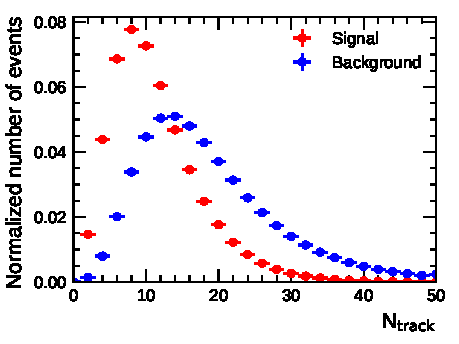
\includegraphics{./figures/rnn/ntrk_1p.pdf}
    \subcaption{Number of tracks associated to a reconstructed 1-prong tau
      candidate.}
    \label{fig:ntracks_tau}
  \end{subfigure}\hfill
  \begin{subfigure}[t]{0.48\textwidth}
    \centering
    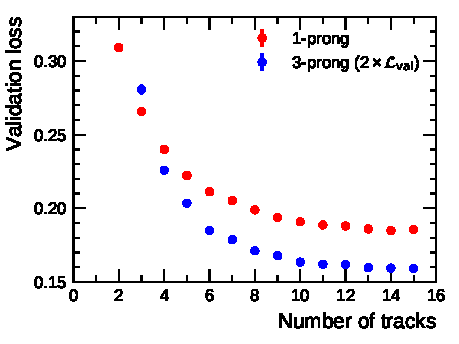
\includegraphics{./figures/rnn/nscan/track_1p_3p.pdf}
    \subcaption{Validation loss as a function of the number of tracks used in
      the model.}
    \label{fig:ntracks_loss}
  \end{subfigure}
  \caption{Number of tracks associated to a tau candidate and their impact on
    the discriminative power of the Track-RNN.}
  \label{fig:rnn_ntracks}
\end{figure}

In Figure~\ref{fig:ntracks_tau} the number of tracks associated to a given tau
candidate is depicted. The number of associated tracks can be large especially
for candidates from background events. For practical purposes the sequence of
tracks is truncated to reduce the memory footprint as well as training and
evaluation time of the network. As the tracks are sorted using a descending
$p_\text{T}^\text{track}$-ordering, truncation will only discard low momentum
tracks. Figure~\ref{fig:ntracks_loss} shows the classification power for
different number of tracks used in the model. The leading six tracks show a
significant impact on the discriminative power of the model. After ten tracks no
further improvement is observed. Therefore, the model will use tracks truncated
after the ten leading tracks in transverse track momentum.

\begin{figure}[htb]
  \begin{subfigure}[t]{0.48\textwidth}
    \centering
    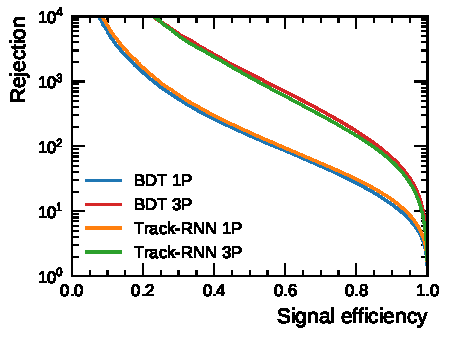
\includegraphics{./figures/rnn/track/roc.pdf}
    \subcaption{ROC-curves for 1-prong (1P) and 3-prong (3P) tau
      identification.}
  \end{subfigure}\hfill
  \begin{subfigure}[t]{0.48\textwidth}
    \centering
    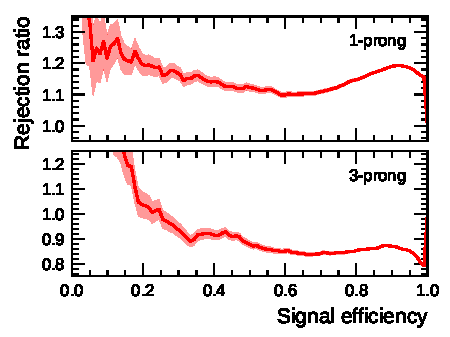
\includegraphics{./figures/rnn/track/ratios.pdf}
    \subcaption{Ratio of rejection of the Track-RNN and the optimised BDT.}
  \end{subfigure}
  \caption{Classification performance of the Track-RNN compared to the optimised
    BDT for tau identification.}
  \label{fig:track_rnn_roc_ratios}
\end{figure}

A comparison of the ROC-curves for the BDT- and RNN-based tau identification is
depicted in Figure~\ref{fig:track_rnn_roc_ratios}. Both the 1- and 3-prong
Track-RNN show a performance similar to the optimised BDT. The 1-prong Track-RNN
shows a small improvement in rejection of \num{10} to \SI{20}{\percent} over the
BDT depending on the signal efficiency. In contrast to this the 3-prong RNN
cannot exceed the performance of the optimised BDT, only capturing \num{80} to
\SI{90}{\percent} of rejection. These results indicate that the available
information in tracks is not fully exploited in the current BDT-based
identification.

\begin{table}[ht]
  \centering
  {\small\begin{tabular}{p{5cm}S[table-format=1.4(4)]S[retain-explicit-plus, table-format=+2.1]}
  \toprule
  {Variables} & {Validation loss} & {Loss increase} \\
  \midrule
  \parbox[c]{\hsize}{Impact parameter \newline $d_0$, $z_0 \sin\theta$}
          & 0.2831 +- 0.0005 & + 48.4 \,\si{\percent} \\[1.2em]
  \parbox[c]{\hsize}{Transverse momentum \newline $p_\text{T}^\text{track}$, $p_\text{T}^\text{jet}$}
          & 0.2410 +- 0.0007 & + 26.3 \,\si{\percent} \\[1.2em]
  \parbox[c]{\hsize}{Angular distance \newline $\Delta \eta$, $\Delta \varphi$}
          & 0.2304 +- 0.0003 & + 20.8 \,\si{\percent} \\[1.2em]
  \parbox[c]{\hsize}{Hits in ID \newline $N_\text{hit}^\text{pixel}$, $N_\text{hit}^\text{SCT}$}
          & 0.2036 +- 0.0013 & + 6.7 \,\si{\percent} \\[1.2em]
  \parbox[c]{\hsize}{Electron probability (TRT) \newline $p_\text{HT}$}
          & 0.1930 +- 0.0004 & + 1.2 \,\si{\percent}\\
  \bottomrule
\end{tabular}

%%% Local Variables:
%%% mode: latex
%%% TeX-master: "../mythesis"
%%% End:
}
  \caption{Variable importance table (1-prong)}
  \label{tab:var_importance_track_rnn}
\end{table}

\todo[inline]{Ultimately these networks cannot be fully understood.}

In Table~\ref{tab:var_importance_track_rnn} the importance of the input
variables is estimated by removing groups of variables and retraining the model.
The increase in validation loss then used to estimate the importance of the
input variables. The impact parameters and transverse momentum have a large
impact on the validation loss. They are essential, as the


Both impact parameters and pt are essential, as they need to be used to identify
tracks originating from the tau vertex and reject low momentum tracks from pileup etc.

- Variable importance

- Correlations



- Working points deferred to later

- What else has been tested? (Bidirectional, stacked)



\begin{figure}[ht]
  \centering
  \begin{subfigure}[t]{0.48\textwidth}
    \centering
    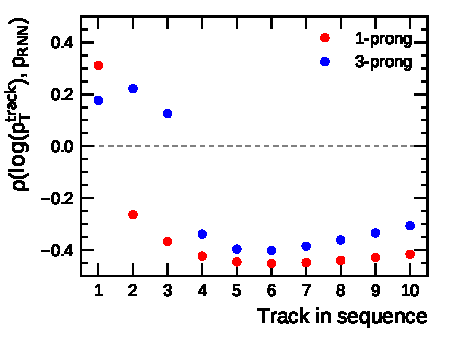
\includegraphics{./figures/rnn/track/pt_corr.pdf}
    \subcaption{}
  \end{subfigure}\hfill
  \begin{subfigure}[t]{0.48\textwidth}
    \centering
    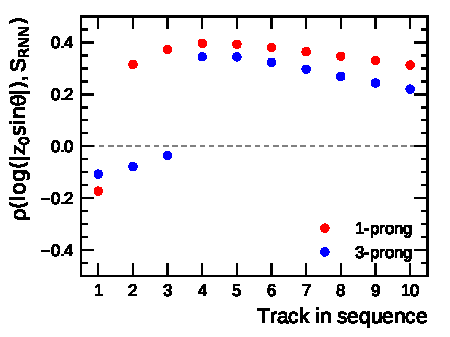
\includegraphics{./figures/rnn/track/z0_corr.pdf}
    \subcaption{}
  \end{subfigure}
  \caption{Correlations}
  \todo[inline]{Explain that $\Delta R$ is similar to $z_0$ i.e.\ close to axis
    for leading 1 or 3 tracks far for rest. Ref to plot in appendix.}
\end{figure}


\todo[inline]{Check whether the missing tau hits in the ID are a problem at
  high-pt.}

\subsection{Cluster-RNN}
\label{sec:rnn_clusters}

\todo[inline]{ROC-Curves}

\todo{Idea is to use cluster moments as a proxy for cell-based variables}

Variable evolution:
\begin{itemize}
\item Energy fractions in PS, EM1, EM2, EM3 (only small improvement)
\item $\Delta R \rightarrow \Delta \phi, \Delta \eta$
\item Importance: 1.\ Direction of the cluster $\Delta \phi, \Delta \eta$; 2.\
  Energy and pt of the jet; 3.\ Cluster moments; 4.\ Energy fractions
\end{itemize}

\begin{figure}[ht]
  \begin{subfigure}[t]{0.48\textwidth}
    \centering
    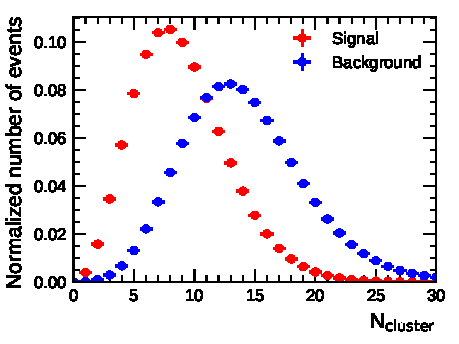
\includegraphics{./figures/rnn/ncls_1p.pdf}
    \subcaption{NCluster for 1-prong taus}
  \end{subfigure}%
  \begin{subfigure}[t]{0.48\textwidth}
    \centering
    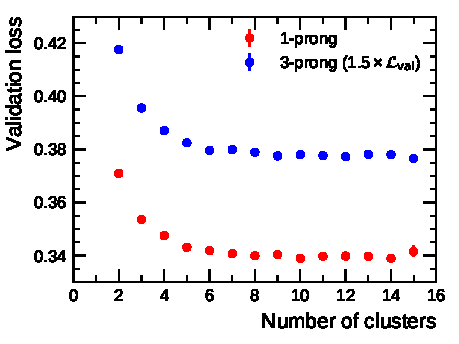
\includegraphics{./figures/rnn/nscan/cluster_1p_3p.pdf}
    \subcaption{Val.\ loss vs.\ nCluster}
  \end{subfigure}
  \caption{Clusters associated with a tau}
  \label{fig:rnn_nclusters}
\end{figure}

\todo{Use 6 clusters}

\begin{itemize}
\item Input variables \& correlation with true class labels. Partial
  dependence plots?
\item Validation loss vs. number of clusters
\item Standalone performance
\end{itemize}


\begin{figure}[ht]
  \begin{subfigure}[t]{0.48\textwidth}
    \centering
    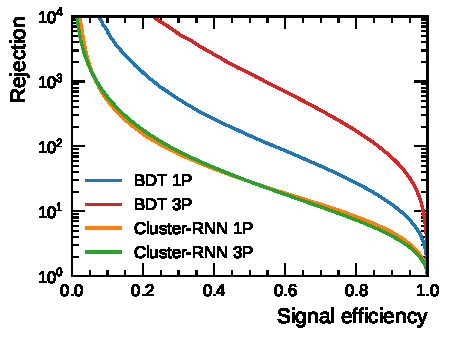
\includegraphics{./figures/rnn/cluster/roc.pdf}
    \subcaption{ROC-curves for 1-prong (1P) and 3-prong (3P) tau
      identification.}
  \end{subfigure}\hfill
  \begin{subfigure}[t]{0.48\textwidth}
    \centering
    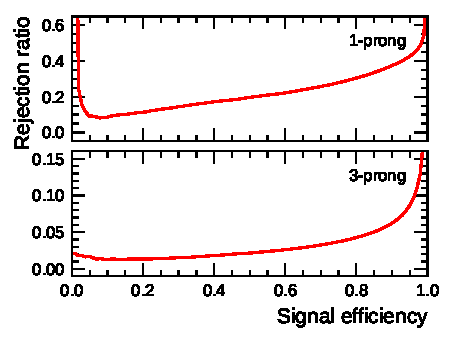
\includegraphics{./figures/rnn/cluster/ratios.pdf}
    \subcaption{Ratio of rejection of the Cluster-RNN and the optimised BDT.}
  \end{subfigure}
  \caption{Classification performance of the Cluster-RNN compared to the optimised
    BDT for tau identification.}
  \label{fig:cluster_rnn_roc_ratios}
\end{figure}

\todo[inline]{Pile-up dependency of RNN vs BDT-ID}

\subsubsection{Di-Tau Identification at the High Luminosity LHC}
\label{sec:hlt_rate_reduction}

The Phase-II upgrade of the LHC called the High Luminosity LHC (HL-LHC) is
foreseen to be finished by 2026. It will increase the instantaneous luminosity
to~\num{5}\,--\,\SI{7.5e34}{\per\square\centi\metre\per\second} at a
centre-of-mass energy
of~$\sqrt{s} = \SI{14}{\TeV}$~\cite{hl_lhc_prelim_design_report}. This
corresponds to a five- to sevenfold increase in luminosity with respect to the
beginning of Run-II and increases the average number of interactions per bunch
crossing to up to \num{200}. The increase in particle density poses a challenge
to the trigger systems and reconstruction algorithms.

An upgrade of the ATLAS trigger with a \emph{Global Trigger System} aims to
provide access to the full calorimeter granularity with topoclustering and jet
finding using iterative jet algorithms in regions of
interest~\cite{phase_2_scoping}. This aims to improve the identification of
physics objects at trigger-level to cope with increasing trigger rates due to
pile-up. Due to the availability of full calorimeter granularity, offline
reconstructed taus can be used to give prospects of the potential performance of
a di-tau trigger in the HL-LHC environment.

A prospective study on the usage of the cluster-based RNN for identification of
taus in a di-tau trigger is given. Offline reconstructed taus are used as an
approximation to the objects at the Phase-II trigger. The study uses simulated
samples of~$\text{Z} / \text{DY} \to \tau \tau$ and dijets at HL-LHC conditions
with centre-of-mass energy~$\sqrt{s}=\SI{14}{\TeV}$ and average interactions per
bunch crossing~$\mu = 200$ (cf.\ Appendix~\ref{app:upgrade_samples}).

The cluster-based RNN identification is retrained on individual tau candidates
in the HL-LHC upgrade samples using the same preselection used for the BDT
identification in Chapter~\ref{sec:bdt} with the exception of any
tracking-related requirements. The leading and subleading tau with respect to
the reconstructed transverse momentum (using Run-II calibrations) are selected
in a given event, while additionally requiring truth-matched hadronic tau decays
for the signal sample. The RNN identification is applied to each tau
individually resulting in two identification scores per event. The leading and
subleading tau~$p_\text{T}$ and identification scores are combined in a logistic
regression to assign a single di-tau identification score to each event.

The accept-rate of \SI{200}{\kilo\hertz} of the higher-level triggers limits the
maximum trigger-rate of the di-tau trigger. Achieving this rate requires
$p_\text{T}$-thresholds on leading and subleading taus as well as application of
the di-tau identification. The thresholds should be kept low to ensure high
signal acceptance for physics analyses. For the purposes of this study a single
cut on the identification score is used to identify di-tau events.

\begin{figure}[htb]
  \centering
  \begin{subfigure}[t]{0.48\textwidth}
    \centering
    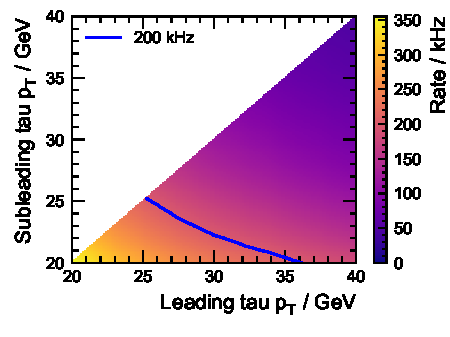
\includegraphics{./figures/rnn/trigger/pt_rate_reg.pdf}
    \subcaption{Trigger-rate after RNN-based identification as a function of
      leading and subleading tau offline $p_\text{T}$-threshold.}
    \label{fig:rate_vs_thresholds}
  \end{subfigure}\hfill
  \begin{subfigure}[t]{0.48\textwidth}
    \centering
    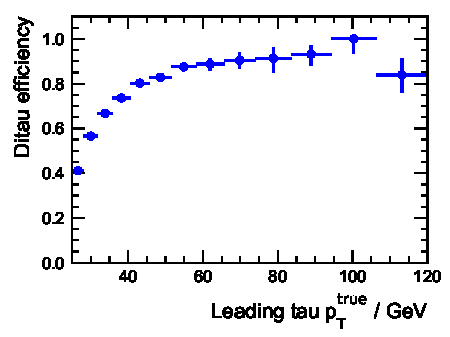
\includegraphics{./figures/rnn/trigger/taueff_reg.pdf}
    \subcaption{Di-tau selection efficiency of RNN-based identification with
      \SI{25}{\GeV} $p_\text{T}$-thresholds with respect to offline
      reconstructed tau lepton pairs measured in $\text{Z} \to \tau\tau$.}
    \label{fig:ditau_trigger_eff}
  \end{subfigure}
  \caption{Feasibility of using TopoClusters for a di-tau trigger at the
    HL-LHC.}
  \label{fig:rnn_ditau_trigger}
\end{figure}

The large dijet production cross section allows the assumption, that all
background events in the simulated sample correspond to a rate equal to the
average bunch crossing rate of~\SI{31.6}{\mega\hertz}. In
Figure~\ref{fig:rate_vs_thresholds} the trigger-rate is shown as a function of
the leading and subleading $p_\text{T}$-thresholds after applying di-tau
identification. The target rate can be achieved with a offline
$p_\text{T}$-threshold of \SI{25}{\GeV} on both taus.
Figure~\ref{fig:ditau_trigger_eff} shows the efficiency of the identification
using the leading and subleading \SI{25}{\GeV} threshold with respect to all
offline reconstructed di-tau pairs. The di-tau efficiency starts to plateau at
true visible transverse momentum~$p_\text{T}^\text{true} > \SI{40}{\GeV}$ of the
leading tau with an efficiency of approximately~\SI{90}{\percent}.

Ref.~\cite{phase_2_scoping} outlines a di-tau trigger with offline
$p_\text{T}$-threshold on the leading and subleading tau of \SI{40}{\GeV} and
\SI{30}{\GeV}, respectively. The approach using the cluster-based RNN
identification achieves the target rate at a reduced $p_\text{T}$-threshold
of~\SI{25}{\GeV}. The efficiency of the selection shows opportunities for
further enhancements by employing a proper tau energy calibration for HL-LHC
conditions and using a more advanced decision threshold for the di-tau
identification. The decision threshold could be loosened with increasing
transverse momentum to ensure a quicker turn-on and full efficiency at
high-$p_\text{t}$.

\subsection{Combined-RNN}
\label{sec:rnn_combined}

\begin{figure}[htb]
  \begin{subfigure}[t]{0.48\textwidth}
    \centering
    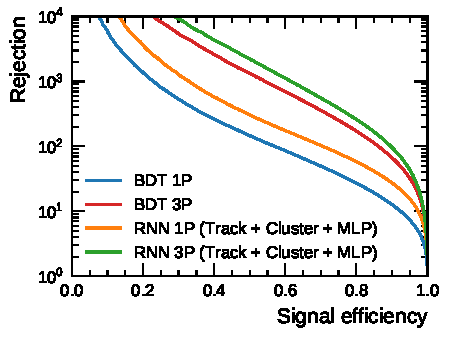
\includegraphics{./figures/rnn/combined/roc.pdf}
    \subcaption{ROC-curves for 1-prong (1P) and 3-prong (3P) tau identification.}
  \end{subfigure}\hfill
  \begin{subfigure}[t]{0.48\textwidth}
    \centering
    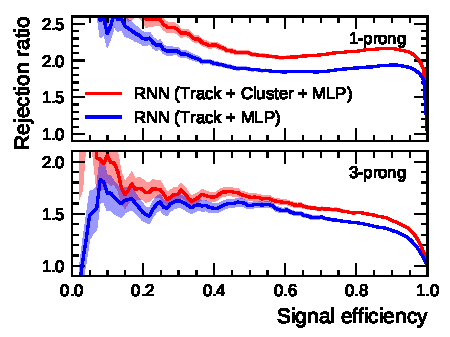
\includegraphics{./figures/rnn/combined/ratios.pdf}
    \subcaption{Ratio of rejection of the combined model and the optimised BDT.}
  \end{subfigure}
  \caption{Classification performance of the combined model compared to the
    optimised BDT for tau identification.}
  \label{fig:roc_combined}
\end{figure}

\begin{figure}[htb]
  \begin{subfigure}[t]{0.48\textwidth}
    \centering
    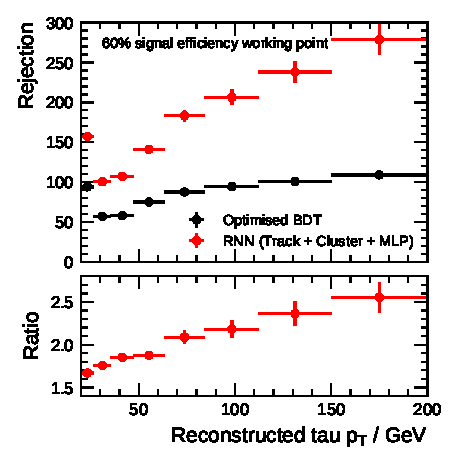
\includegraphics{./figures/rnn/combined/rnn_tight_1p.pdf}
    \subcaption{1-prong}
  \end{subfigure}\hfill
  \begin{subfigure}[t]{0.48\textwidth}
    \centering
    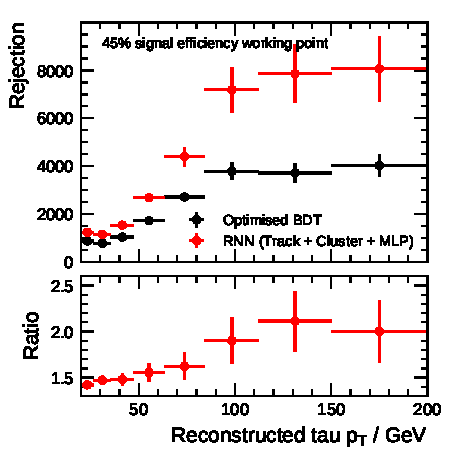
\includegraphics{./figures/rnn/combined/rnn_tight_3p.pdf}
    \subcaption{3-prong}
  \end{subfigure}
  \caption{Background rejection at the tight working point as a function of the
    reconstructed tau $p_\text{T}$ at tau energy scale for the BDT- and
    RNN-based identification.}
  \label{fig:combined_working_points}
\end{figure}



%%% Local Variables:
%%% mode: latex
%%% TeX-master: "mythesis"
%%% End:
